\documentclass[12pt,a4paper]{article}
\usepackage[utf8]{inputenc}
\usepackage[T1]{fontenc}
\usepackage{amsmath}
\usepackage{amsfonts}
\usepackage{amssymb}
\usepackage{graphicx}
\usepackage{physics}
\usepackage{cite}
\usepackage{caption}
\usepackage{subcaption}
\usepackage{hyperref}
\usepackage{comment}

\linespread{1.2}
\usepackage[a4paper,top=3cm,bottom=3cm,left=3cm,right=3cm]{geometry}

\title{Prove Max-Ergotropy}
\author{}

\begin{document}
	\maketitle


	For now i'll work with direct Lanczos diagonalization. \\
	We break the symmetry with a little field h and then we calculate on two sites in the middle of the chain:
	\begin{itemize}
		\item $E(\rho)/2|\epsilon_0|$
		\item $E(\rho^{pass})/2|\epsilon_0|$
		\item $E(\rho^{a-pass})/2|\epsilon_0|$
	\end{itemize}
	\begin{itemize}
		\item Ergotropy = $E(\rho)/2|\epsilon_0| -E(\rho^{pass})/2|\epsilon_0|$
		\item Anti-Ergotropy $E(\rho^{a-pass})/2|\epsilon_0|-E(\rho)/2|\epsilon_0|$
		\item Max-Ergotropy $E(\rho^{a-pass})/2|\epsilon_0|-E(\rho^{pass})/2|\epsilon_0|$
	\end{itemize} 
 It's important to normalize everything  since the quantities depend strongly on the Hamiltonian eigenvalues\\
 
	We also calculate some known quantities :
	\begin{itemize}
		\item Purity
		\item Entropy
		\item Concurrence
	\end{itemize}

	\newpage
	\section{Experimental trials, broken symmetry}

	\begin{figure}[h]
		\centering
		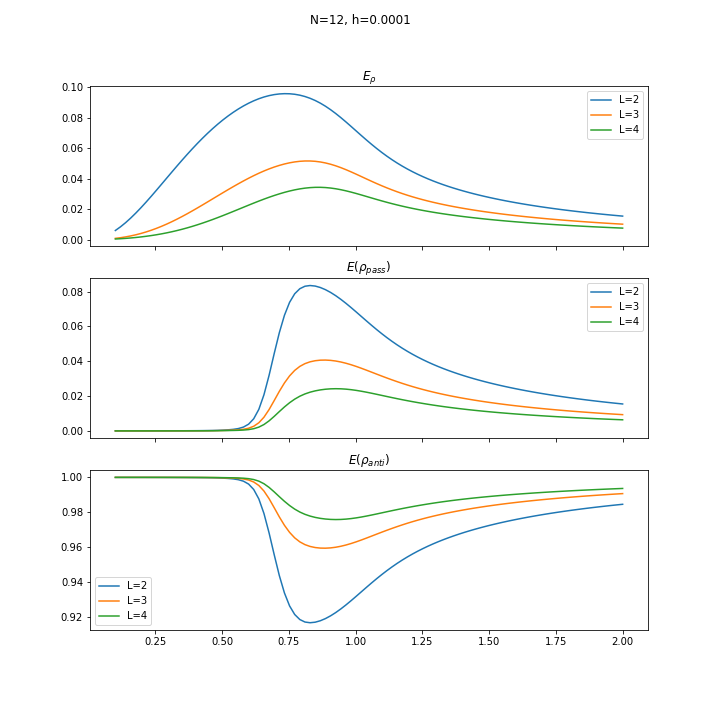
\includegraphics[width=\linewidth]{h1_rhos}
		\caption{}
		\label{fig:h1rhos}
	\end{figure}
	\begin{figure}[h]
		\centering
		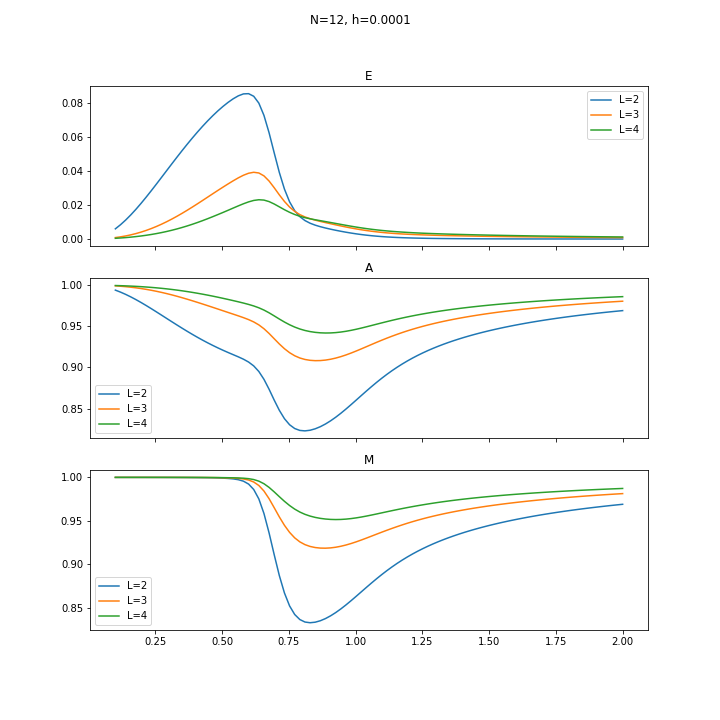
\includegraphics[width=\linewidth]{h1_ergos}
		\caption{}
		\label{fig:h1ergos}
	\end{figure}
	\begin{figure}[h]
		\centering
		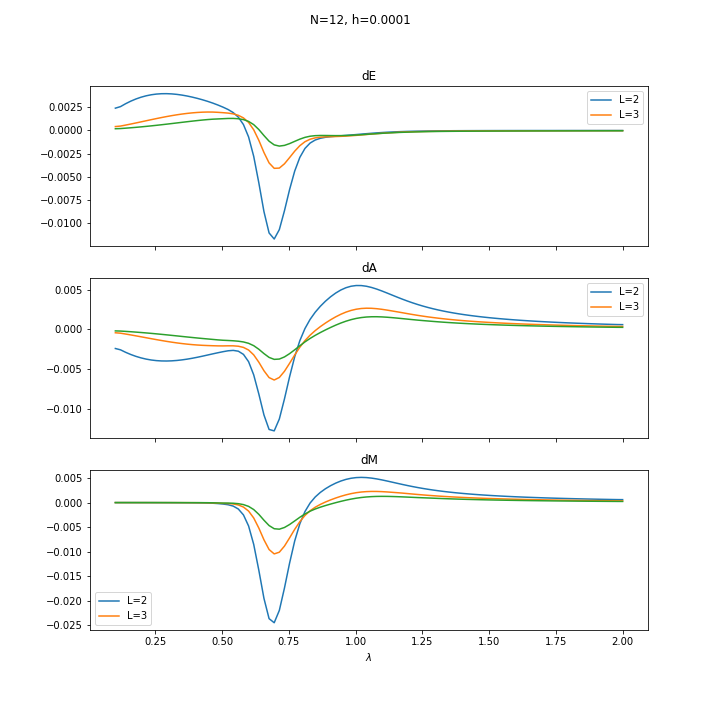
\includegraphics[width=\linewidth]{h1_dergos}
		\caption{}
		\label{fig:h1dergos}
	\end{figure}	
	
	\begin{figure}[h]
		\centering
		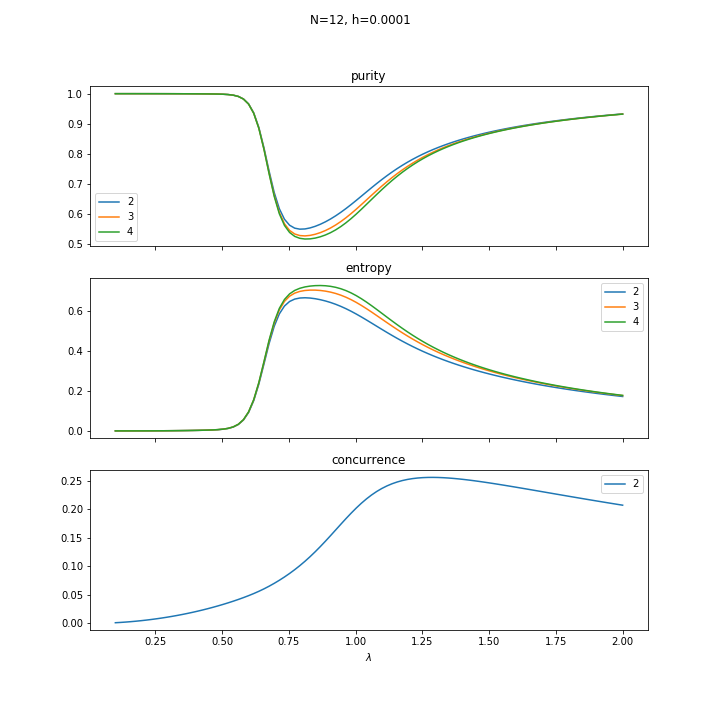
\includegraphics[width=\linewidth]{h1_quantities}
		\caption{}
		\label{fig:h1quantities}
	\end{figure}
	
	
	\clearpage
	\section{Experimental trials, preserved symmetry}

	\begin{figure}[h]
		\centering
		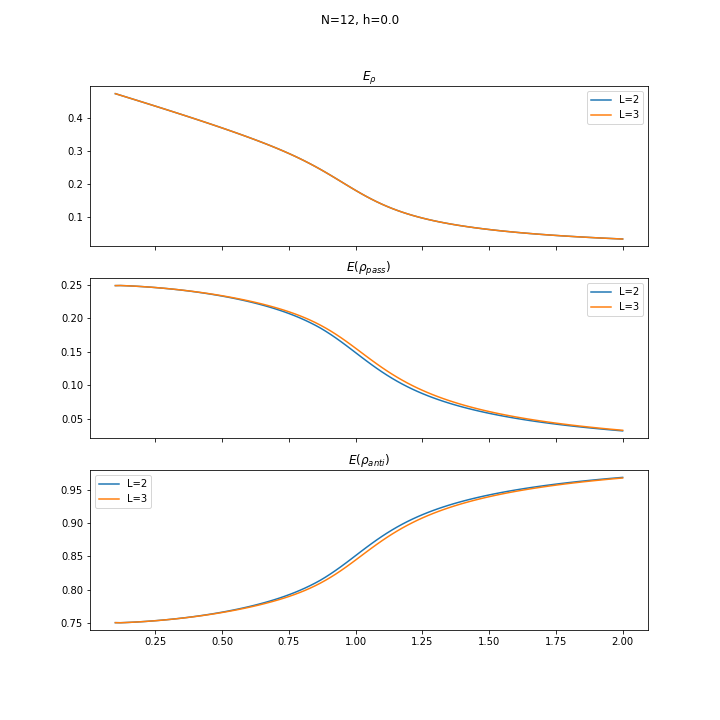
\includegraphics[width=\linewidth]{h0_rhos}
		\caption{}
		\label{fig:h0rhos}
	\end{figure}
	\begin{figure}[h]
		\centering
		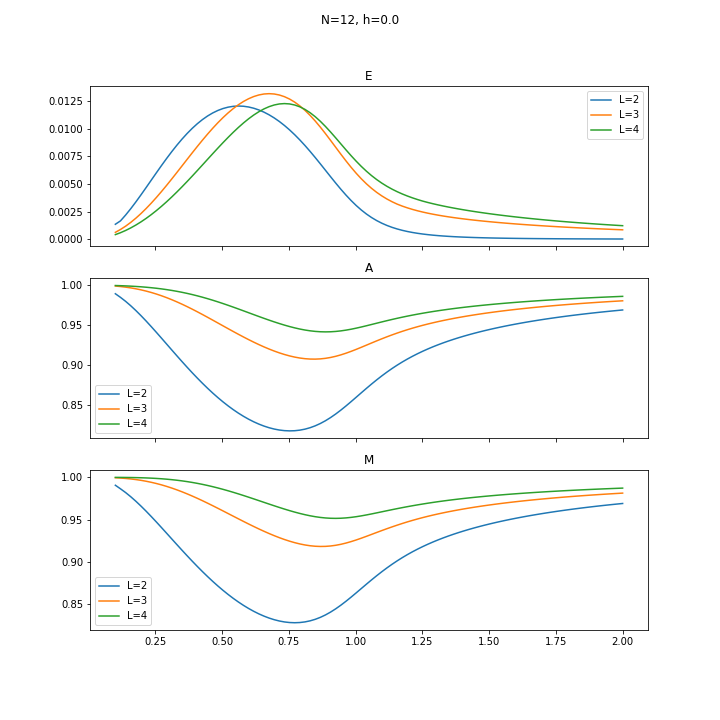
\includegraphics[width=\linewidth]{h0_ergos}
		\caption{}
		\label{fig:h0ergos}
	\end{figure}
	\begin{figure}[h]
		\centering
		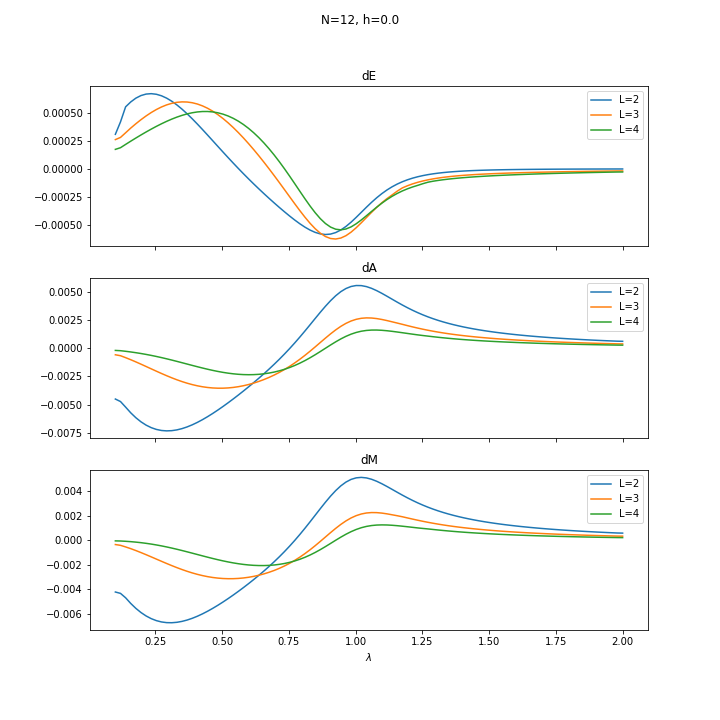
\includegraphics[width=\linewidth]{h0_dergos}
		\caption{}
		\label{fig:h0dergos}
	\end{figure}	
	
	\begin{figure}[h]
		\centering
		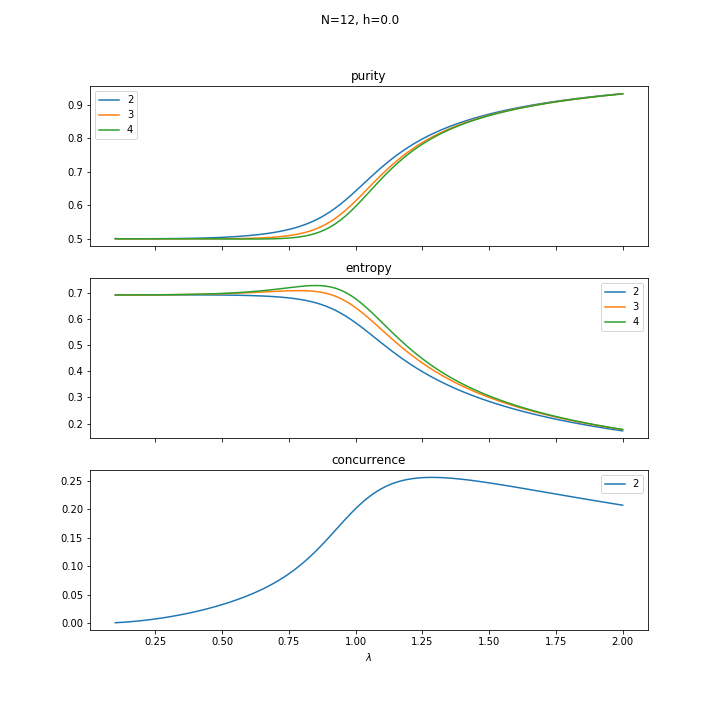
\includegraphics[width=\linewidth]{h0_quantities}
		\caption{}
		\label{fig:h0quantities}
	\end{figure}
	
	
	
	
	
	\clearpage
	\section{Theoretical calculations, preserved symmetry}
		\begin{figure}[h]
		\centering
		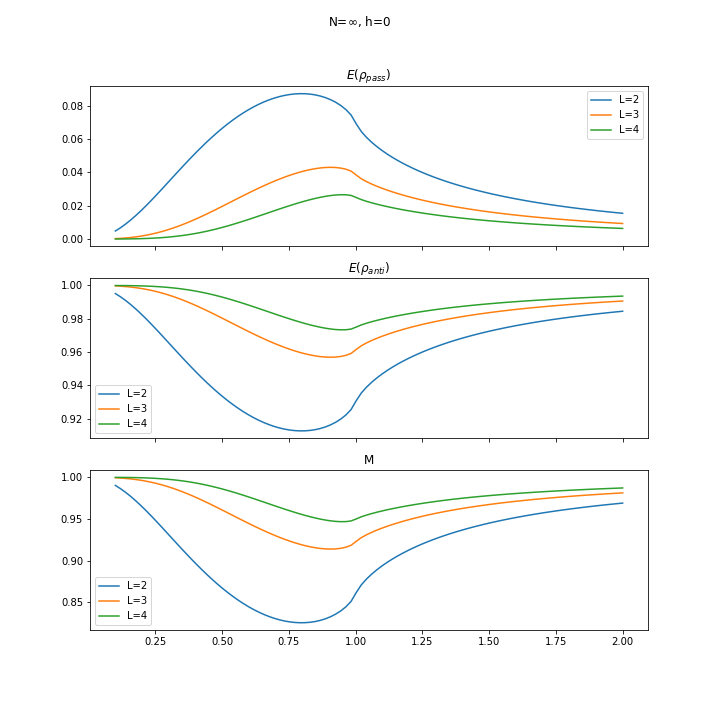
\includegraphics[width=\linewidth]{ergostheo}
		\caption{}
		\label{fig:ergostheo}
	\end{figure}	
	
	\begin{figure}[h]
		\centering
		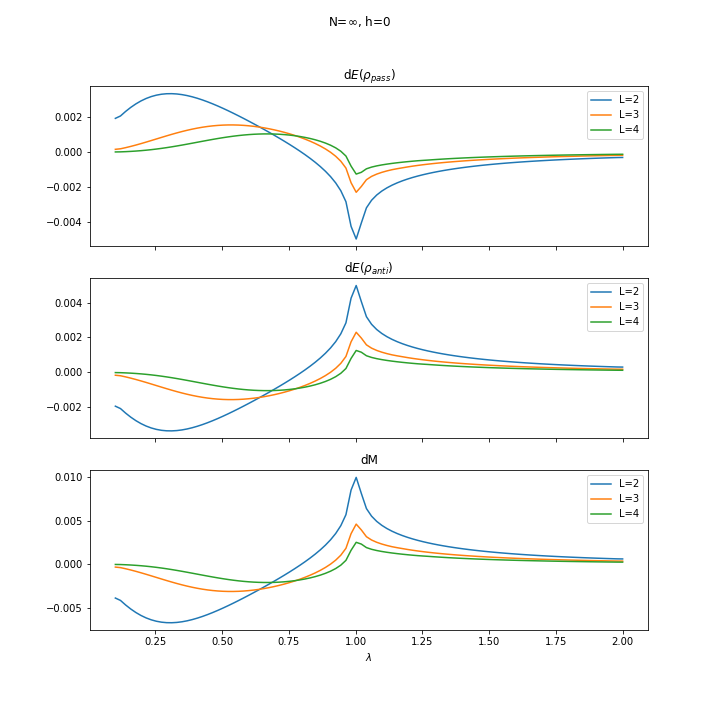
\includegraphics[width=\linewidth]{d_ergostheo}
		\caption{}
		\label{fig:dergostheo}
	\end{figure}
	\begin{figure}[h]
		\centering
		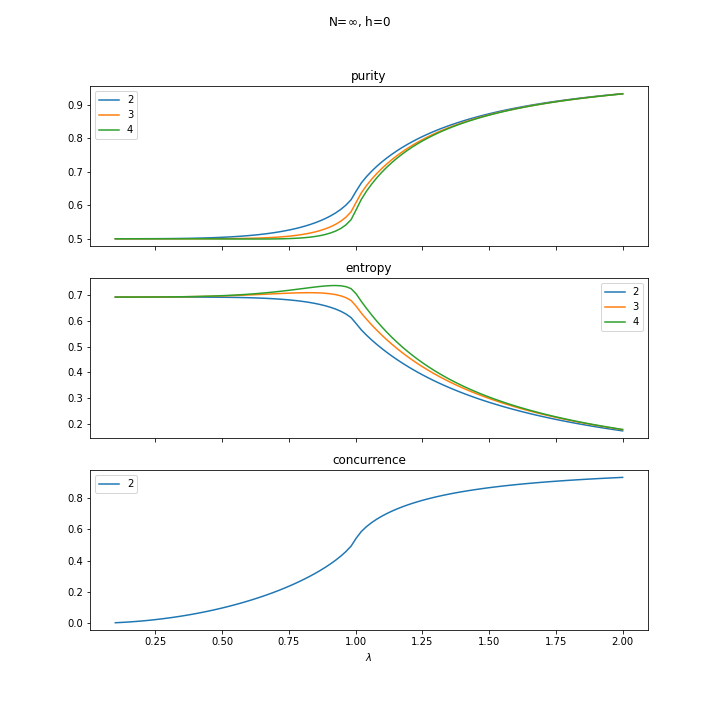
\includegraphics[width=\linewidth]{theo_quantities}
		\caption{}
		\label{fig:theoquantities}
	\end{figure}



\clearpage


	
\end{document}